\documentclass[11pt]{scrartcl}
\usepackage[pdftex]{graphicx}
\usepackage{asymptote}
%\documentclass[11pt]{amsart}
\usepackage[sexy]{evan}
\usepackage{amsmath, amssymb, listings, color, amsthm, amsfonts}
\usepackage[margin=1in]{geometry}
\usepackage{fancyhdr}
\allowdisplaybreaks 
\usepackage{subfiles}
%\renewcommand{\familydefault}{\sfdefault}
\renewcommand\vec{\mathbf}
\usepackage{hyperref}
\usepackage{physics}
\usepackage{circuitikz}
\usepackage{wrapfig}

\newcommand{\thiscirc}[1]{
\texttt{#1} \hfill \begin{circuitikz} \draw
(0,0) node[ #1 ] {};%(2,0); 
\end{circuitikz} {\hspace{5mm}}}


\newcommand{\bipole}[1]{
\texttt{#1} \hfill \begin{circuitikz} \draw
(0,0) to[ #1 ] (2,0); 
\end{circuitikz} {\hspace{5mm}}}
\title{Lagrangian Handout}
\begin{document}
\maketitle

\subsection*{Acknowledgments}
\textsc{Thanks} to Tarun Agarwal, QiLin Xue, Kushal Thaman, and Sanjay Suresh for providing helpful comments and suggestions. 
\section{Introduction}
This handout\footnote{This handout was created with $\texttt{evan.sty}$, a $\text\LaTeX$ package created by \href{https://github.com/vEnhance/dotfiles/blob/master/texmf/tex/latex/evan/evan.sty}{Evan Chen}.} is not meant to provide a rigorous introduction to lagrangian mechanics presented in undergraduate physics. However, it will go through a practical step by step process such that a person who understands the theory and examples presented in this handout will be able to solve olympiad physics problems through the usage of lagrangian formalism. For those who want more in depth discussions about lagrangian and hamiltonian mechanics, here are a few other resources available:
\begin{itemize}
    \ii \textit{Introduction to Classical Mechanics: With Problems and Solutions} by David J. Morin.
    \ii \textit{Classical Mechanics} by Herbert Goldstein.
    \ii \textit{Classical Mechanics} by John R. Taylor.
    \ii \href{https://www.damtp.cam.ac.uk/user/tong/dynamics/two.pdf}{David Tong's Notes} on Lagrangian formalism. 
\end{itemize}
\section{Basic Theorems and Identities}
\begin{definition}
The lagrangian of a system is defined by 
\[\mathcal{L} \equiv T - V\]
where $T$ is the kinetic energy and $V$ is the potential energy.
\end{definition}
\begin{definition}
The generalized coordinate $q$ describes how the entire system moves with respect to a certain
coordinate. For example, the generalized coordinate of a ball rolling down a ramp would be the distance that the ball travels parallel to the ramp.
\end{definition}
As to their name, generalized coordinates are coordinates for \textbf{every} aspect of a system. This includes coordinates such as translational components $x$ and angular components $\theta$. The generalized coordinate can be collected as an $n$ dimensional vector 
\[\vec{q} = \begin{pmatrix}
q_1 \\
q_2 \\
\vdots \\
q_n
\end{pmatrix}
\]
however this vector doesn't have much meaning as each component of the vector may have different units. 
\begin{theorem}
\label{thm:1}
To find the acceleration $\ddot{q}$ of the generalized coordinate $q$, we can express the potential energy $V$ of the system as a function $V\left(q\right)$ of $q$ and the kinetic energy in the form $T=\frac{1}{2}\mathcal{M}\dot{q}^2$ where the coefficient $\mathcal{M}$ is the effective mass. We then see that the acceleration of the system will be defined as
\[\ddot{q}=-V'\left(q\right)/\mathcal{M}.\]
\end{theorem}
\begin{proof}
By conservation of energy, 
\[\frac{1}{2} \mathcal{M}\dot{q}^2 + V (q) = \text{const.}\]
differentiating with respect to $q$ gives us 
\[\mathcal{M}\dot{q}\ddot{q} + V' (q)\dot{q} = 0.\]
Dividing over by $\dot{q}$ and then isolating $\ddotq$ gives us 
\[\ddot{q} = -V' (q)/\mathcal{M}\]
\end{proof}
Note that theorem \ref{thm:1} only works in a \textbf{system with one degree of freedom}.
\begin{definition}
The action of a system\footnote{Note that the action $\mathcal{S}$ is a functional integral which means that it depends on the functions $\vec{q}$ has.} along a path $\vec{q}(t)$ between two times $t_1$ and $t_2$ is defined as 
\[\mathcal{S} = \int_{t_1}^{t_2}\mathcal{L}(q_i, \dot{q}_i, t)dt.\]
Quantitatively, the action has the units of $E\times t$ where $E$ is the energy and $t$ is the time. 
\begin{theorem}[Hamilton's Principle]
The evolution $\vec{q}(t)$ of a system between two times $t_1$ and $t_2$ is the path that yields a stationary value of the action. 
\end{theorem}
The motivation for Hamilton's principle is discussed in Appendix A\ref{appendix:a}, but for now, we can just take this principle to be for granted. 
\end{definition}
\begin{theorem}[Euler Lagrange Equations]
The Euler-Lagrange equations are given by 
\[\frac{d}{dt}\left(\pdv{\mathcal{L}}{\dot{q}}\right) = \pdv{\mathcal{L}}{q}\]
where $\dot{q}$ and $q$ are the generalized velocity and coordinate respectively.
\end{theorem}
The Euler-Lagrange equations are really important because they hold in \textbf{all} frames. With Newton's laws, we would have to modify the forces to include other ones such as fictitious forces in non-inertial frames but with the Euler-Lagrange equations we only have to write the kinetic and potential energy of the system in any frame and we will get our desired equation of motion. Why this is true is because the Euler-Lagrange equations are derived by Hamilton's principle (which we will do below) which doesn't depend on what reference frame the evolution of $\vec{q} (t)$ happens in. 
\begin{proof}
\label{proof:1}
Note that readers who just want to know how the Euler-Lagrange equations are applied can skip this proof. 

The Euler-Lagrange equations are a consequence of Hamilton's principle or to be more specific, the Euler-Lagrange relations come when $\vec{q}(t)$ yields a stationary value (i.e an extrema) of the action $S$. We can use variational analysis to derive the integral of $\mathcal{S}$. Let us assume that the function $q$ yields a stationary value of $\mathcal{S}$. Then any slight variation of $q$ must either increase or decrease $q$ depending on whether it is a minima or maxima of $\mathcal{S}$. Let us then consider the function 
\[q_{\varepsilon} (t) \equiv q(t) + \varepsilon \eta (t)\]
where $\varepsilon$ is really small and $\eta (t)$ is a function that satisfies $\eta (t_1) = \eta(t_2) = 0$. Let us then define $\mathcal{S}_{\varepsilon}$ to be such that 
\[\mathcal{S}_{\varepsilon} = \mathcal{S} (q_{\varepsilon} (t), \dot{q}_{\varepsilon} (t), t).\]
For $q$ to yield a stationary value of $\mathcal{S}$, we require that there is no change in $\mathcal{S}_{\varepsilon}$ in the first order of $\varepsilon$. In other words, we need to find how $\mathcal{S}_{\varepsilon}$ depends on $\varepsilon$. By differentiating, we yield 
\[\pdv{}{\varepsilon} \mathcal{S}_{\varepsilon} = \dv{}{\varepsilon} \int_{t_1}^{t_2} \mathcal{L} (q_{\varepsilon}, \dot{q}_{\varepsilon}, t) \dd t = \int_{t_1}^{t_2} \pdv{\mathcal{L}_{\varepsilon}}{\varepsilon}\dd t.\]
It follows that the total derivative is given by 
\[\pdv{\mathcal{L}_{\varepsilon}}{\varepsilon} = \sum_{i=1}^{n}\pdv{\mathcal{L}}{q_i}\dv{q_i}{\varpesilon} = \pdv{\mathcal{L}_{\varepsilon}}{q_{\varepsilon}}\dv{q_{\varepsilon}}{\varepsilon} + \pdv{\mathcal{L}_{\varepsilon}}{\dot{q}_{\varepsilon}}\dv{\dot{q}_{\varepsilon}}{\varepsilon} + \pdv{\mathcal{L}_{\varepsilon}}{t}\dv{t}{\varepsilon}.\]
The last term cancels out and we are left with 
\[\pdv{}{\varepsilon}\mathcal{S}_{\varepsilon} = \int_{t_1}^{t_2}\left(\pdv{\mathcal{L}_{\varepsilon}}{q_{\varepsilon}}\dv{q_{\varepsilon}}{\varepsilon} + \pdv{\mathcal{L}_{\varepsilon}}{\dot{q}_{\varepsilon}}\dv{\dot{q}_{\varepsilon}}{\varepsilon}\right)\dd t.\]
Remember that from what we have established, 
\[\dv{q_{\varepsilon}}{\varepsilon} = \eta (t), \quad \pdv{\dot{q}_{\varepsilon}}{\varepsilon} = \dot{\eta} (t)\]
and once again, we can rewrite our integral to be 
\[\pdv{}{\varepsilon}\mathcal{S}_{\varepsilon} = \int_{t_1}^{t_2} \left(\eta (t)\pdv{\mathcal{L}_{\varepsilon}}{q_{\varepsilon}} + \dot\eta (t) \pdv{\mathcal{L}_{\varepsilon}}{\dot{q}_{\varepsilon}}\right)\dd t.\]
We can apply integration by parts on the second term of the integrand to result in 
\[\int \dot\eta (t) \pdv{\mathcal{L}_{\varepsilon}}{\dot{q}_{\varepsilon}} \dd t = \eta (t) \pdv{\mathcal{L}_{\varepsilon}}{\dot{q}_{\varepsilon}} - \int \left(\dv{}{t} \pdv{\mathcal{L}_{\varepsilon}}{\dot{q}_{\varepsilon}}\right)\eta (t) \dd t.\]
Replacing this into the second part of our previous equation leaves us with 
\[\pdv{}{\varepsilon} \mathcal{S}_{\varepsilon} = \left.\eta (t) \pdv{\mathcal{L}_{\varepsilon}}{\dot{q}_{\varepsilon}}\right|_{t_1}^{t_2} + \int_{t_1}^{t_2}\left(\pdv{\mathcal{L}_{\varepsilon}}{q_{\varepsilon}} - \dv{}{t}\pdv{\mathcal{L}_{\varepsilon}}{\dot{q}_{\varepsilon}}\right)\eta (t) \dd t.\]
The first term in this expression cancels out to zero and since we require the derivative of $\mathcal{S}_{\varepsilon}$, we require the integral to evaluate to zero (at $\varepsilon = 0$) which means that 
\[\dv{}{t}\left(\pdv{\mathcal{L}}{\dot{q}}\right) = \pdv{\mathcal{L}}{{q}}\]
and hence the Euler-Lagrange equations are proved!\footnote{This is still not the most general proof available. For one, we have assumed that $\mathcal{L}$ is twice differentiable. We could go about proving the Euler-Lagrange equations for this less general case but this is not what this handout is for. Luckily, mathematicians and physicists have deduced that Euler-Lagrange equations still work in that case.}
\end{proof}

Sometimes when we are applying to the Euler-Lagrange equation for more than one generalized coordinate, we will result in \textbf{coupled differential equations} which are two or more equations that depend on each other as a function of time. For example, 
\begin{align*}
    M\ddot{x}_1 &= -kx_1 + \kappa x_2 \\
    M\ddot{x}_2 &= \kappa x_1 - kx_1
\end{align*}
are coupled differential equations. In a coupled differential equation we generally have three quantities. One is the $M$ matrix which is a $n\times n$ dimensional matrix that determines the mass distribution of all the $n$ coupled differential equations we have. It has $m_j$ in the $j$th row and the $j$th column with zeroes everywhere else. In other words, $M$ is determined as 
\[M = \begin{pmatrix}
m & 0 & \dots & 0 \\
0 & m_2 & \dots & 0 \\
\vdots & \vdots & \ddots & \vdots \\
0 & 0 & \dots & m_n
\end{pmatrix}\]
We also define the $K$ matrix as an $n\times n$ matrix that has a coefficient $K_{jk}$ in its $j$th row and $k$th column:
\[K = \begin{pmatrix}
K_{11} & K_{12} & \dots & K_{1n} \\
K_{21} & K_{22} & \dots & K_{2n} \\
\vdots & \vdots & \ddots & \vdots \\
K_{n1} & K_{n2} & \dots & K_{nn}
\end{pmatrix}\]
Finally, we write the column vector $X$ which has $x_j$ in it's $j$th row:
\[X = \begin{pmatrix}
x_1 \\
x_2 \\
\vdots \\
x_n
\end{pmatrix}\]
We now introduce our theorem that we use to solve coupled oscillators:
\begin{theorem}
If we have a $n\times n$ dimensional matrix $M$ and $K$ and a $n$ dimensional vector $X$ which described all $n$ coupled differential equations in a system of the form of 
\[M\ddot{X} = -KX,\]
our solution can be described as 
\[\det (M^{-1} K - \omega^2 I) = 0\]
where $I$ is the identity\footnote{The identity matrix is simply just a matrix that has $1$s in all of it's eigenvalues.} matrix.
\end{theorem}
\begin{proof}
We move into complex notation $Z \equiv e^{i (\omega t + \phi)}A$ where $A$ is a column vector $(A_1, A_2, A_3)$ and $X_j = \Re (Z_j)$. Our equation of motion then transforms into 
\[M\ddot{X} = -KX\implies M\ddot{Z} = -KZ.\]
Substituting our solution of $Z$, we result in 
\[M\omega^2 Z = KZ \implies M\omega^2 A = KA\]
dividing the equation by $M$ and factoring out $A$ results in 
\[(M^{-1}K - \omega^2 I) A = 0.\]
To get a solution, we then need to solve 
\[\det (M^{-1} K - \omega^2 I) = 0.\]
\end{proof}
The solutions for the frequencies of these coupled differential equations upon using this identity is called the \textbf{eigenfrequencies} of the system. If you feel a bit lost after this introduction to coupled oscillators, don't fret as we'll go over a couple examples on solving them after applying the Euler-Lagrange equations. 
\begin{exercise}
Solve the previous coupled differential equations
\begin{align*}
    M\ddot{x}_1 &= -kx_1 + \kappa x_2 \\
    M\ddot{x}_2 &= \kappa x_1 - kx_1
\end{align*}
for their eigenfrequencies.
\end{exercise}
\newpage 
\section{Examples}
There will be many examples from physics olympiads of how lagrangian formalism is used. This is mainly because not many people are aware of how this technique is used in olympiads.
\begin{example}[2019 EuPhO]
Three small identical balls (denoted as A, B, and C) of mass $m$ each are connected with two massless rods of length $\ell$ so that one of the rods connects the balls A and B, and the other rod connects the balls B and C. The connection at the ball B is hinged, and the angle between the rods can change effortlessly. The system rests in weightlessness so that all the balls lie on one line. The ball A is given instantaneously a
velocity perpendicular to the rods. 

Find the minimal distance $d$ between the balls A and C during the subsequent motion of the system. Any friction is to be neglected.
\end{example}

\begin{soln}
If there are no constraints, there are $j = 6$ degrees of freedom as each mass can freely move as $(x_A, y_A, x_B, \dots)$. However, as there are 2 rods, they constrain each of the 3 masses, so there are only $3$ degrees of freedom. Furthermore, if we fix the center of mass, then that gets rid of another degree of freedom. This leaves us with only 2 degrees of freedom to consider which greatly simplifies the problem. As $AB = AC = \ell$, the moment where $A$ and $C$ are the closest will be when the mass-rod system forms an isoceles triangle. We will proceed by defining our 2 generalized coordinates as $q \in (\varphi, d)$ where $2\varphi$ is the separating angle, and $d$ is the distance between $A$ and $C$. In the center of mass frame, the system moves with a velocity $v_{\text{CM}} = mv/3m = v/3$ in the negative $Y$-axis. Thus, $A$ moves with a velocity of $\frac{2}{3}v$ and $B$ and $C$ move with a velocity of $-\frac{v}{3}$ in the negative $Y$-direction initially. Thus, the total initial energy of the balls is 
\[E = \frac{1}{2}mv^2 \left(\frac{4}{9} + \frac{1}{9} + \frac{1}{9}\right) = \frac{1}{3}mv^2.\]

\noindent As the center of mass frame is inertial, conservation laws of energy, momentum, and angular momentum hold, we will equate this energy to a generalized energy of the system in its isosceles triangle form. 
Let the center of mass be point $M$ as shown in the figure to the right. Let $h$ be the height of the center of mass. The velocity $v_A$ can be written as the vector sum of vertical $\dot h$ velocity and rotational $h \dot \varphi$ velocity. This will be the velocity corrections due to the change in velocity in the center of mass frame and thus there will be the same ratios as presented in the beginning. One can express the velocities of balls $A$ and $C$ also in terms of the vector sum of $\dot{\tilde{d}}$ and $\tilde d\dot \varphi$ where $\tilde{d} = d/2$. Hence, we write 
\[\mathcal L = \frac{1}{2}m \left(\frac{4}{9} \left(\dot h^2 + h^2 \dot \varphi^2\right) + \frac{2}{9}h^2\dot \varphi^2 + 2 \dot{\tilde{d}}^2 + 2\tilde{d}^2\dot\varphi^2\right) = \frac{1}{3}mv^2.\]
At the closest distance, $\dot{\tilde{d}} = 0 = \dot h$ which means that $2\tilde{d}^2\dot\varphi^2 + \frac{2}{3}h^2 \dot\varphi^2 = \frac{2}{3}mv^2$. We can try to find an expression for $\dot \varphi (t)$ by noting that the rate in change of the lagrangian with respect to $\dot \varphi$ remains constant with time. This is because $\mathcal L$ doesn't necessarily depend on $\varphi$ throughout. Note that at $t = 0$, $\dot \varphi = v\ell/2$. Then:
\[\pdv{\mathcal L}{\dot \varphi} = \frac{1}{2}m \left(\frac{8}{9}h^2\dot\varphi + \frac{4}{9}h^2\dot\varphi + 4\tilde{d}\dot\varphi\right) = \text{const}.\]
Removing all constant factors and equating to the intial rate of change in energy thus tells us that 
\[\left(\frac{1}{3}h^2 + \tilde{d}\right)\dot \varphi = \ell^2 \cdot \frac{v\ell}{2} \implies \dot\varphi = \frac{v\ell}{2 \left(\frac{1}{3}h^2 + \tilde{d}\right)}.\]
Further simplifying by plugging into our other equation and cancelling out $v$ yields:
\[\tilde{d} = \sqrt{\frac{5}{8}}\ell \implies d = \sqrt{\frac{5}{2}}\ell!\]
\end{soln}
\begin{example}[2017 China Semi-Finals]
A solid cylinder of mass $m$ and radius $r$ rests on the inside of a thin-walled cylinder of mass $M$ and radius $R.$ The solid cylinder is made to oscillate around the equilibrium position. Assuming $g$ to be the gravitational acceleration, find the frequency of this oscillation for the following cases:
\begin{enumerate}
\item The large cylinder is fixed, and the small cylinder rolls without slipping in the bottom of the cylinder.
\item The large cylinder is permitted to rotate about an axis through its fixed center, and the small cylinder rolls without slipping in the bottom of the cylinder.
\end{enumerate}
\end{example}
\begin{soln}
We start this solution by thinking of each individual types of energy.
\begin{enumerate}
    \item Let the total angle the smaller solid cylinder move through an angle $\varphi$ with respect to the walls of the larger hollow cylinder and let $\theta$ be the angle with respect to the vertical that the smaller cylinder moves through. 
    \begin{center}
        \begin{asy}
        size(8cm);
        import olympiad;
draw(arc((0,0),1,0,-180));
draw(circle((0.38, -0.7), 0.2));
draw(circle((0, -0.8), 0.2), dotted);
dot((0.38, -0.7));
dot((0, -0.8));
draw((0, -0.8) -- (0, 0) -- (0.38, -0.7));
draw(anglemark((0, -0.8), (0, 0), (0.38, -0.7)));
label("$\theta$", (0.03, -0.23), SE);
dot((0.38 - 0.2*sqrt(3)/2, -0.7 - 0.2*1/2));
dot((0.38 + 0.1, -0.7 - 0.175));
markscalefactor = 0.01;
draw(anglemark((0.38 - 0.2*sqrt(3)/2, -0.7 - 0.2*1/2), (0.38, -0.7), (0.38 + 0.1, -0.7 - 0.175)));
draw((0.38 - 0.2*sqrt(3)/2, -0.7 - 0.2*1/2) -- (0.38, -0.7) -- (0.38 + 0.1, -0.7 - 0.175), dotted);
label("$\varphi$", (0.38, -0.77), SW);
        \end{asy}
    \end{center}
    The translational velocity of the center of mass is proportional to the time derivative of the change of $\theta$, i.e. $v = (R - r) \dot\alpha$. The cylinder also rotates with time. Finding the angular velocity is a little tricky as the reference line passing through the inner cylinder center to point of intersection of the inner and larger cylinder rotates with time. Thus, $\omega_C = \dot\phi = \frac{d}{dt} (\varphi - \theta)$. Thus the angular velocity of the cylinder can be characterizes as 
    \[\omega = \frac{R - r}{r}\dv{\theta}{t} = \frac{v}{r}.\]
    Noting that the moment of inertia of a cylinder through its axis is $I = \frac{1}{2}mr^2$, we can write the lagrangian as 
    \[\mathcal{L} = T - V = \frac{1}{2}m(R - r)^2 \dot\theta^2 + \frac{1}{4}mr^2 \dot\varphi^2 + mg (R - r)\cos \theta\]
    and using our constraint condition, we can write 
    \[\mathcal{L} = \frac{3}{4}m(R - r)^2 \dot\theta^2 + mg(R - r)\cos\theta.\]
    Applying the Euler-Lagrange equation for a general coordinate $\theta$ then tells us that 
    \[\dv{}{t} \left(\pdv{\mathcal{L}}{\dot\theta}\right) = \pdv{\mathcal{L}}{\theta}\implies \frac{3}{2}m (R - r)^2 \ddot\theta = -mg (R - r)\sin \theta.\]
    Rearranging, gives us a standard differential equation for harmonic oscillations:
    \[\ddot\theta = -\frac{2}{3}\left(\frac{g}{R - r}\right)\theta \implies \omega = \sqrt{\frac{2}{3}\left(\frac{g}{R - r}\right)}\]
    by using the small angle approximation $\sin\theta \approx \theta$.
    \item By adding the kinetic and potential components of the larger mass $M$ and applying lagrangian fomalism once again (you are advised to work this out) we result in the differential equation 
    \[\ddot\theta = -\left(\frac{2mg (R - r)}{2m (R - r)^2 + MR^2}\right)\theta = 0\implies \omega = \sqrt{\frac{2mg (R - r)}{2m (R - r)^2 + MR^2}}.\]
\end{enumerate}
Now that we are done solving this problem, I want to talk about how this solution could have gone wrong. If we had used a constraint, for example, a rolling without slipping constraint, then we have reduced the number of degrees of the system from $(x, \theta, \varphi)\to (x, \theta)$. This would lead to an incorrect result, because the path from one place to the other becomes more general. In other words, \textbf{do not use the Euler-Lagrange equations if you reduce a two degree system to one degree by using constraint conditions} as they will lead to the wrong answer. If you find that you can reduce the number of degrees to one by using constraint conditions, it might be easier to theorem \ref{thm:1} instead. NB! Most olympiad problems try to make the problem presentable such that there is only one degree of freedom. 
\end{soln}
\begin{example}[2018 $F=ma$ B, 1998 BAUPC]
Two particles of mass $m$ are connected by pulleys as shown.
\begin{center}
    \includegraphics[width=6cm]{88ED384A-7503-491B-86AF-BC22A8F1DD2F.png}
\end{center}
The string passes over a set of massless pulleys of negligible size. The masses are at rest a distance $\ell$ away from the pulleys. The mass is given a very small velocity such that it swings back and forth with an amplitude $\epsilon$ (where $\epsilon \ll \ell$). It turns out that after a long time, one of the masses will eventually rise up and hit its pulley. Which mass hits its pulley?
\end{example}
\begin{soln}
The Lagrangian of this system after a small deviation $\theta$ of the left mass is given by 
\[\mathcal{L} = \frac{1}{2}m\dot{\ell}^2 + \frac{1}{2}m (\dot\ell^2 + \ell^2\dot\theta^2) - mg\ell + mg\ell\cos\theta.\]
Applying the Euler-Lagrange equations for each respective generalized coordinate gives us
\begin{align*}
    \frac{d}{dt}\left(\pdv{\mathcal{L}}{\dot\ell}\right) &= \pdv{\mathcal{L}}{\ell}\implies 2m\ddot\ell = m\ell\dot\theta^2 - mg(1 - \cos\theta) \\
    \frac{d}{dt}\left(\pdv{\mathcal{L}}{\dot\theta}\right) &= \pdv{\mathcal{L}}{\theta}\implies m\ell^2\ddot{\theta} = -mg\ell\sin\theta
\end{align*}
If we do a  small angle approximation of 
\[\sin\theta \approx \theta, \quad \cos\theta \approx 1 - \frac{1}{2}\theta^2\]
we result in the equations 
\begin{align*}
    \ddot\ell &= \frac{1}{2}\ell\dot\theta^2 - \frac{1}{4}g\theta^2 \\
    \ddot\theta &= -\frac{g}{\ell}\theta
\end{align*}
Our second equation is a simple harmonic oscillation equation and tells us that the mass has a function of $\theta (t)$ of 
\[\theta (t) = \epsilon \cos (\omega t + \varphi)\]
where $\omega \equiv \sqrt{g/\ell}$. This means that upon substitution with 
\[\dot\theta (t) = \epsilon \omega \sin (\omega t + \varphi)\]
we result in the equation 
\begin{align*}
\ddot\ell &= \frac{1}{2}\ell \epsilon^2 \omega^2 \sin^2 (\omega t + \varphi) - \frac{1}{4}\epsilon^2 g\cos^2 (\omega t + \varphi) \\
\ddot \ell &= \frac{1}{2}\epsilon^2 g\left(\sin^2 (\omega t + \varphi) - \frac{1}{2}\cos^2 (\omega t + \varphi)\right)
\end{align*}
Averaging this function for a long time, tells us that 
\[\ddot\ell_{\text{avg}} = \frac{1}{8}\epsilon^2 g\]
which is positive and means that the right mass slowly oscillates upwards vertically\footnote{Note that this is applicable for only the first moment as we assumed that $\ell$ is constant. However, after the first moment the motion will continue it keeps getting pulled forward.} and will hit the pulley first.
\end{soln}

\begin{example}[2003 EstAcadPhO]
Two coaxial rings of radius $R = 10\;\mathrm{cm}$ are placed to a distance $L$ from each other. There is a soap film connecting the two rings as shown in figure. Derive a differential equation describing the shape $r(z)$ of the film, where $r$ is the radial distance of the film from the symmetry axis, as the function of the distance $z$ along the axis. Show that $\cosh (x)$ is one of its solutions. When the distance between rings is slowly increased, at a certain critical distance $L_0$, the soap film breaks. Find $L_0$.
\begin{center}
    \includegraphics[width=5cm]{kaldathermo.png}
\end{center}
\end{example}
\begin{soln}
We want to minimize the energy of the soap film $E=S\gamma$. This is achieved when the area $S$ is at a minimum. The area is:
$$S=\int_{-L/2}^{L/2} 2\pi r\sqrt{1+r'^2} dr$$We want to minimize $r\sqrt{1+r'^2}$ which we can take to be our Lagrangian. We can apply the Euler Lagrange equations, except instead of $r$ being dependent on time, it's dependent on $x$. This equivalent is:
\begin{align*}
\frac{d}{dx}\left(\frac{\partial L}{\partial r'}\right)&=\frac{\partial L}{\partial r} \\
\frac{d}{dx}\left(2\pi r \frac{r'}{\sqrt{1+r'^2}}\right) &= 2\pi\sqrt{1+r'^2}
\end{align*}which can be simplified to:
$$1+r'^2=Ar^2$$where $A=1/r_0^2$. The solution is well known. Motivated by the fact that $1+\sinh^2x=\cosh^2x$, we can guess the solution:
$$r(x)=r_0\cosh (x/r_0).$$
Therefore, 
$$x=r_0\cosh^{-1}\left(\frac{r}{r_0}\right) \implies r = r_0\cosh\left(\frac{x}{r_0}\right)$$If the separation is $L$, we get:
$$R = r_0\cosh(L/2r_0) \implies L = 2r_0\cosh^{-1}\left(R/r_0\right)$$where $R$ is the radius of the ends. Finding the maximum value of $L$ by using a calculator gives us $13.3\;\mathrm{cm}$.
\end{soln}

\begin{example}[Pan Pearl River Delta Physics Olympiad]
As shown, a block of mass $m$ is connected to a spring of force constant $k$ on the smooth slope (inclination angle $\theta$) of a wedge of mass $M$ placed on a smooth floor. Given a small disturbance to the block and the system starts to oscillate. During the oscillation motion, the block keeps in touch with the slope and the wedge maintains contact with the floor. Find the oscillation frequency. 
\begin{center}
    \includegraphics[width = 6cm]{F0768028-9ADA-4047-AE98-867627605677.png}
\end{center}
\end{example}
\begin{soln}
Let the length of the spring that connects the mass $m$ on top of the ramp at a certain time $t$ be $\ell$. The mass $m$ will then have coordinates of time as 
\[(x, y)_{\text{CM}} = (x + \ell \cos \theta, h - \ell \sin\theta).\]
If we take $x$, $\dot{x}$, and $\dot\ell$ to be the generalized coordinates, the kinetic energy of this system is then 
\[T = \frac{1}{2}M\dot{x}^2 - \frac{1}{2}m \left((\dot{x} + \dot\ell\cos \theta)^2 + (\dot\ell\sin\theta)^2\right).\]
The potential energy on the other hand is 
\[V = -\frac{1}{2}k (\ell - \ell_0)^2 mg (h - \ell \sin \theta)\]
where $\ell_0$ is the relaxed spring length. We can then write the lagrangian as 
\[\mathcal{L} = T - V = \frac{1}{2}M\dot{x}^2 + \frac{1}{2}m \left((\dot{x} + \dot\ell\cos \theta)^2 + (\dot\ell\sin\theta)^2\right) + \frac{1}{2}k (\ell - \ell_0)^2 - mg (h - \ell \sin \theta).\]
Rewriting this tells us that 
\[\mathcal{L} = \frac{1}{2}(m + M)\dot{x}^2 + \frac{1}{2}m\dot\ell^2 + m\dot\ell\dot{x}\cos\theta - \frac{1}{2}k (\ell  - \ell_0)^2 - mg(h - \ell \sin\theta).\]
We can then apply the Euler-Lagrange equations for each respective generalized coordinate:
\begin{align*}
    \frac{d}{dt}\left(\pdv{\mathcal{L}}{\dot{x}}\right) &= \pdv{\mathcal{L}}{x}\implies (m + M)\ddot{x} + m\ddot\ell \cos \theta = 0 \\
    \frac{d}{dt}\left(\pdv{\mathcal{L}}{\dot{\ell}}\right) &= \pdv{\mathcal{L}}{\ell} \implies m\ddot\ell + m\ddot{x}\cos\theta = k(\ell_0 - \ell) - mg\sin\theta
\end{align*}
We can find the equilibrium position of the mass by balancing forces. We have by Newton's laws that 
\[mg\sin\theta - k(\ell^{\prime} - \ell_0) = 0\implies \ell^{\prime} = \frac{mg\sin\theta}{k} - \ell_0.\]
We then set the position of the mass $\ell$ as 
\[\ell = \ell^{\prime} + \frac{mg\sin\theta}{k} + d.\]
By rewriting our two equations above, we yield two coupled differential equations:
\begin{align*}
    (m + M)\ddot{x} + m\ddot\ell^{\prime} \cos\theta &= 0 \\
    m\ddot{x}\cos\theta + m\ddot\ell^{\prime} + k\ell^{\prime}&= 0
\end{align*}
By applying the matrix identity 
\[\det (M^{-1}K - \omega^2 I) = 0\]
we yield the following determinant 
\[\begin{vmatrix}
-(m + M)\omega^2 & -m\omega^2\cos\theta \\
-m\omega^2\cos\theta & k - m\omega^2
\end{vmatrix}
= 0.\]
Upon applying the determinant and solving for $\omega$ we yield 
\[\omega = \sqrt{\frac{k (m + M)}{m (M + m\sin^2\theta)}}.\]
\end{soln}
Lagrangian analysis is also helpful in other fields apart from mechanics. One nice field that it is used in is Circuitry. To be more specific, when the problem asks you to calculate the eigenfrequencies (natural frequencies) of the circuit. 

\newpage 
\section{When to use Lagrangian Formalism}

After all this discussion about lagrangian formalism, there still remains the question on when you \textit{should} use lagrangian formalism and what benefits it has over other techniques. First, let us think about the benefits and advantages of lagrangian formalism:
\begin{itemize}
    \ii Usually when using lagrangian formalism, we have the advantage of there being scalar quantities that we have to worry about instead of vector quantities that are usually related with Newtonian mechanics. 
    \ii Lagrangian formalism is the most useful when there is only conservative forces and no non-conservative forces involved (such as friction). You can still use the lagrangian in cases with friction but it gets much more messy. 
    \ii Lagrangian formalism is very useful when there are a lot of constraints. The more constraints there are in a system, the easier it becomes to write the lagrangian and the harder it becomes to the Newtonian form. 
    \ii As you will see in the problems, lagrangian formalism is very accessible in the way that you can use it for aspects other than mechanics i.e electric circuits and optics. 
    \ii In many olympiad problems, it becomes the easiest to use lagrangian formalism when there is more than one degree of freedom. 
\end{itemize}
Therefore, when there are a lot of constraints involved in a system, and there is more than one degree of freedom, you can start thinking about applying the lagrangian. Many times, the lagrangian technique can be overkill, however, the lagrangian technique also requires the least thinking to apply. 
\newpage 
\section{Problems}
\begin{problem}[2015 $F=ma$]
A U-tube manometer consists of a uniform diameter cylindrical tube that is bent into a U shape. It is originally filled with water that has a density $\rho_w$. The total length of the column of water is $L$. Ignore surface tension and viscosity. The water is displaced slightly so that one side moves up a distance $x$ and the other side lowers a distance $x$. Find the frequency of oscillation.
\end{problem}
\begin{problem}[2019 $F=ma$]
A uniform rope of length $L$ and mass $M$ passes over a frictionless pulley, and hangs with both ends at equal heights. If one end is pulled down a distance $x$ and the rope is released, what will be the acceleration of the end of that instant?
\end{problem}
\begin{problem}[Krotov, Kalda]
A small block with mass m lies on a wedge with angle $\alpha$ and mass $M$. The block is attached to a rope pulled over a pulley attached to the tip of the wedge and fixed to a horizontal wall (see the figure). Find the acceleration of the wedge. All surfaces are slippery (there is no friction).
\begin{center}
    \includegraphics[width=6cm]{krotov.jpg}
\end{center}
\end{problem}

\begin{problem}
A laser beam propogates through a spherically symmetric medium surrounding a metal sphere of radius $R$. Refractive index of the medium varies with distance $r$ from the center O of the sphere according to the law $\mu (r) \propto r$. Here $R \ll r < \infty$. 

The laser beam makes an angle of $\phi$ with a radial line at point P, which is a distance $r_0$ away from O. What is the minimum distance from the surface of the sphere that the beam can reach?
\end{problem}

\begin{problem}[Krotov, Kalda]
Two slippery ($\mu = 0$) wedge-shaped inclined surfaces with equal tilt angles $\alpha$ are positioned such that their sides are parallel, the inclines are facing each other and there is a little gap in between (see fig.). On top of the surfaces are positioned a cylinder and a wedge-shaped block, whereas they are resting one against the other and one of the block’s sides is horizontal. The masses are, respectively, $m$ and $M$. What accelerations will the cylinder and the block move with? Find the reaction force between them.
\begin{center}
    \includegraphics[width=6cm]{wedgecylinder.jpg}
\end{center}
\end{problem}
\begin{problem}[1984 IPhO]
\href{https://www.ioc.ee/~kree/students/iphoTable/files/ipho/1984_Sweden_p2.pdf}{Problem 2}
\end{problem}
\begin{problem}[Kalda]
An empty cylinder with mass $M$ is rolling without slipping along a slanted surface, whose angle of inclination is $\alpha = 45^{\circ}$. On its inner surface can slide freely a small block of mass $m = M/2$. What is the angle $\beta$ between the normal to the slanted surface and the straight line segment connecting the centre of the cylinder and the block?
\begin{center}
    \includegraphics[width=6cm]{rollingcylinder.png}
\end{center}
\end{problem}
\begin{problem}[2020 OPhO]
In this problem, we will explore the true gravitational model of the earth, not the one that is claimed in most textbooks. Contrary to popular belief, the Earth is a flat circle of radius $R$ and has a uniform mass per unit area $\sigma$. The Earth rotates with angular velocity $\omega$.

\begin{enumerate}[label=(\alph*)]
\item A pendulum of length $\ell$ that is constrained to only move in one plane is placed on the ground at the center of the Earth. The pendulum has more than one angular frequency of small oscillations. Find the value of each angular frequency of small oscillations $\Omega (0), \Omega_1 (0), ...$ in terms of $\sigma$, $\omega$, $\ell$, and physical constants and the equilibrium angle $\theta, \theta_1, ...$ that the frequency occurs at. Assume for all parts that $\ell \ll R$.
\vspace{3mm}

\noindent An equilibrium angle corresponds to the angle with respect to the vertical where there is an equilibrium point.

\item The entire pendulum is moved a horizontal distance $r \ll R$ away from the center of the Earth. It is oriented so that it is constrained to only move in the radial direction. Now, find the new angular frequency $\Omega (r)$ of small oscillations about the lowest equilibrium point in terms of the given parameters, assuming that $\omega^2 r$ is much less than the local gravitational acceleration.
\end{enumerate}
Note that the parts that don't use lagrangian formalism have been taken out. You can view the whole problem \href{https://opho.physoly.tech/static/files/opho2020_invi.pdf}{here}.
\end{problem}
\begin{problem}[1971 IPhO]
A wedge with mass $M$ and acute angles $\alpha_1$ and $\alpha_2$ lies on a horizontal surface. A string has been drawn across a pulley situated at the top of the wedge, its ends are tied to blocks with masses $m_1$ and $m_2$. What will be the acceleration of the wedge? There is no friction anywhere.
\begin{center}
    \includegraphics[width=6cm]{ipho.jpg}
\end{center}
\end{problem}

\begin{problem}
A point mass on the end of a light string rotates as a conical pendulum with an angular velocity $\Omega$. The string is inclined at an angle $\varphi$ to the vertical. If the motion is slightly disturbed, find the value of the angular frequency of small oscillations.
\end{problem}

\begin{problem}[1986 IPhO]
\href{https://www.ioc.ee/~kree/students/iphoTable/files/ipho/1986_UnitedKingdom_p3.pdf}{Problem 3}, (note that this problem is about coupled oscillators instead of applying lagrangian formalism).
\end{problem}

\begin{problem}
Find the natural frequencies of the circuit given below 
\begin{center}
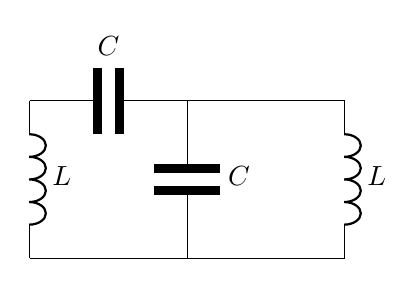
\begin{tikzpicture}[transform shape]
\ctikzset{label/align = smart}
\draw (0, 2) to [american inductor, l=$L$] (0, 0);
\draw (0, 2) to [capacitor, l=$C$, line width=1.5] (2, 2);
\draw (2, 2) to [capacitor, l=$C$, line width=1.5] (2, 0);
\draw (0, 0) -- (4, 0);
\draw (4, 2) to [american inductor, l=$L$] (4, 0);
\draw (4, 2) -- (2, 2);
\end{tikzpicture}
\end{center}
\end{problem}

\begin{problem}[2012 Physics Cup]
Determine all the eigenfrequencies (=natural frequencies) of the circuit shown in Figure. You may assume that all the capacitors and inductances are ideal, and that the following strong inequalities are satisfied: $C_1 \ll C_2$, and $L_1 \ll L_2$. Note that your answers need to be simplified according to these strong inequalities.
\begin{center}
    \includegraphics[width=5cm]{physicscup.jpg}
\end{center}
\end{problem}

\begin{problem}[2021 Physics Cup]
Find all non-trivial natural oscillation frequencies for a regular octagon made from eight homogeneous bars of mass $m$ and length $l$. While the bars are rigid, the connectors connecting two neighboring bars are such that the angle $\varphi$ between the bars can be changed without any friction, but a returning torque $T = k\left(\varphi - \frac{3}{4}\pi\right)$ will appear at the joint as soon as the angle departs from its equilibrium value $\frac 34\pi$.  Indicate how many linearly independent oscillation modes correspond to each of these frequencies. Consider only planar oscillation modes, i.e. modes by which the bars move only in the plane of the octagon.
\\
\\
\textit{Note:} The usage of lagrangian formalism in this problem is not part of the intended solution, and requires quite a bit of mathematical work. The problem is put here, in case you are interested in doing the math and bashing out a problem fully. It would be recommended to read more advanced theory such as construction of energy matrices to finish it this way. Either way, the intended solution to this problem has a good connection with coupled oscillations (refer to problem 5.9), so it is nice to try it. 
\end{problem}
\newpage 
\section{Appendix A: Virtual Work and Hamilton's Principle}
\label{appendix:a}
Hamilton's principle may have come out of the blue, so in this section we will discuss the basis for how this principle came about. A lot of Hamilton's principle was based on the work done by D'Alembert and the principle of virtual work. Some of you may not be familiar with the principle of virtual work, so we can introduce that principle here. Consider a system that is in equilibrium. If we displace this system by a small virtual displacement\footnote{The displacement is virtual because no displacement actually happens. We are considering that this displacement happens with no time passing so we can consider the physics that happens because of this.} $\delta \vec{r}_i$, it will result in a force $\vec{F}_i$ acting onto system and doing work at different amounts for different times. We consider the \textbf{virtual work} done on this particle $\vec{F}_i \cdot \delta \vec{r}_i$. The system is in equilibrium, or in other words, $\sum_{i}\vec{F}_i = 0$ and since the virtual displacement means that no resultant force actually happens on the particle, we require that 
\[\sum_{i} \vec{F}_i \cdot \delta \vec{r}_i = 0\]
when the system is in equilibrium. 
\begin{theorem}[Virtual Work]
If we consider a virtual displacement $\delta \vec{r}_i$ of a system in equilibrium, we require by the principle of virtual work that 
\[\sum_{i} \vec{F}_i \cdot \delta \vec{r}_i = 0.\]
\end{theorem}
In D'Alembert's work, he considered when a system was accelerating. When an object is accelerating, we add in an "inertial force" equal to $-ma$, then the virtual displacement of the particle would again have zero dot product with $F=ma$. This gives
\[(F(q(t)) - ma) \cdot \delta q(t) = 0.\]
Similar to the proof\ref{proof:1} of the Euler-Lagrange equations, we once again use variational analysis in this system. Let us consider a small displacement $\varpesilon$, it is then written that 
\[q_{\varepsilon} = q(t) + \varepsilon \delta q (t).\]
where $\delta q(t_1) = \delta q(t_2) = 0$. Using D'Alembert's generalized principle of virtual work between two times $t_1$ and $t_2$ tells us that 
\[\int_{t_1}^{t_2} [F(q(t)) - m\ddot{q} (t) ]\cdot \delta q(t) \dd t = 0\]
for all $\delta q (t)$. Noting that $F = -\grad V$ means that 
\[ \int_{t_1}^{t_2} [-\grad V(q(t)) \cdot \delta q(t) - m\dot{q} (t) \cdot \dot{q}(t)]\dd t,\]
and we can rewrite 
\[\grad V (q(t)) \cdot \delta q(t) = \left.\grad V(q) \cdot \dv{q_{\varepsilon}(t)}{\varepsilon}\right|_{\varepsilon = 0} = \left.\dv{}{\varepsilon}V(q_{\varepsilon} (t)\right|_{\varpesilon = 0} = \delta V(q(t))\]
and 
\[\delta (\dot{q} (t))^2 = 2\dot{q} (t) \cdot \delta \dot{q} (t)\]
so that our integral is written as 
\[\int_{t_1}^{t_2} \left(-\delta V(q(t)) + \frac{1}{2}m\delta (\dot{q}(t))^2\right)\dd t = 0.\]
This integral can then be rewritten as 
\[\delta \left(\int_{t_1}^{t_2}[T(q(t)) - V(q(t))]\dd t\right) = 0.\]
This itself is the action 
\[\mathcal{S} = \int_{t_1}^{t_2} \mathcal{L} (q, \dot{q} (t), t) \dd t\]
which implies that 
\[\delta \mathcal{S} = 0\]
which is Hamilton's principle itself! Joseph-Louis Lagrange produced this type of calculation and published it in his own paper and that is why today the lagrangian is known as $\mathcal{L} \equiv T - V$. From this proof, you can see that Hamilton's principle is a generalization of nature itself and today remains as one of the most beautiful principles of all time. 
\end{document}
